% Activate the following line by filling in the right side. If for example the name of the root file is Main.tex, write
% "...root = Main.tex" if the chapter file is in the same directory, and "...root = ../Main.tex" if the chapter is in a subdirectory.
 
%!TEX root =  TNTinderSee.tex

Das Multibeam erledigte einen großen Teil unserer Arbeit, doch trotzdem stellten wir uns die Frage was wohl wäre, wenn sich noch Bomben oder ähnliches auf dem Meeresboden befinden, wir allerdings an dieser Stelle zufällig genau nicht vermessen. Mithilfe von Jens Greinert kamen wir dann auf die Idee, an bestimmten Punkten auf unserer Strecke Wasserproben zu nehmen. 

Der Vorteil der Wasserproben war natürlich, dass sich nicht genau an der Stelle wo wir sie entnommen hatten eine Bombe hätte sein müssen, sondern es reichte wenn sich Sprengstoffähnliche Verbindungen im Wasser befinden, vielleicht auch von weiter weg.  

\subsubsection{Technische Beschreibung und Durchführung an Board}
Die Wasserproben waren relativ simpel aufgebaut. Wir hatten ein Plastikrohr mit Deckeln, welche mithilfe von zwei Gummis offen gehalten wurden. Das Rohr wurde ins Wasser gelassen, jeweils abgestimmt auf die Tiefe etwa einen Meter oben dran, sodass aufgewirbelter Dreck oder Algen nicht im Weg waren. Sobald es sich an der richtigen Stelle befand, wurde ein kleines metallenes \emph{Engelchen} dem Seil an welchem das Rohr war entlang, in die Tiefe geschickt. Das Engelchen war aufgrund von seinem Material relativ schwer, wodurch sich die Gummis an dem Rohr lösten und die Deckel zu gingen. Danach musste die Probe nur noch hoch gezogen werden.

Sobald sich die Probe wieder auf dem Boot befand konnten wir weiter fahren zu dem nächsten Standpunkt wo eine hohe Wahrscheinlichkeit bestand etwas zu finden. Auf dem Boot ging dann allerdings erst die richtige Arbeit los, nämlich aus der rohen Wasserprobe eine zu machen, aus welcher man auch Informationen ziehen konnte. An dem Rohr befand sich ein kleines Ventil, wodurch wir das Wasser langsam und kontrolliert in einen Messbecher laufen lassen konnten. Mit viel Feingefühl versuchten wir genau 1000ml zu bekommen. Es würde keinen großen Unterschied machen, wenn es mehr oder weniger wäre, allerdings hat uns das einiges an Rechnen erspart. 

Das abgemessene Wasser wurde anschliessend durch einen selbst gebauten Trichter in ein \emph{Blood Bag} gefüllt, solche wie man auch in Operationen finden würde, um normalerweise Blut zu lagern. In unserem Fall war dies allerdings nur ein Zwischenschritt. 
An dem dem Blood Bag befestigten wir einen kleinen Schlauch befestigtenmit einem Filter, durch das das Wasser gelassen wurde. Im Anschluss an den Filter, welcher lediglich Schmutzpartikel aus dem Wasser filterte, befand sich ein kleines Teströhrchen mit einer Art Granulat. Dieses war nach unten hin offen, da das fertig durchgelaufene Wasser unbrauchbar für uns war, weshalb wir es einfach langsam abtropfen lassen konnten.

Die eigentliche Magie war nun das geschehen in dem Granulat. Dieses war nämlich absichtlich dafür, um schadstoffähnliche Verbindungen aus dem Wasser zu filtern und zu speichern. Dazu kam noch die Anforderung, dass man möglichst genau einen Liter durch das Teströhrchen laufen lassen sollte, um einen möglihst genauen Vergleich ziehen zu können, wo sich eventuell mehr oder weniger Verbindungen befanden. Natürlich ist es auch möglich anhand von anderen Stoffen im Wasser zu bestimmen, wie viel Milliliter Wasser man genau benutzt hat, doch für uns war es so am einfachsten. 

\subsubsection{Probenpräparation am GEOMAR}
Die Teströhrchen haben wir anschließend mit ins Geomar nach Kiel genommen. Dort haben wir die Proben für den Ionenchromatographen präpariert, indem eine definierte Menge von destilliertem Wasser über das Granulat haben laufen lassen. Anschließend wurden die Proben mit einem Verdünnungsmittel auf 2ml aufgefüllt. Diese nun fertige Probe wurde dann auf Rückstände sprengstofftypischer Verbindungen analysiert.
\begin{figure}[]
    \centering
    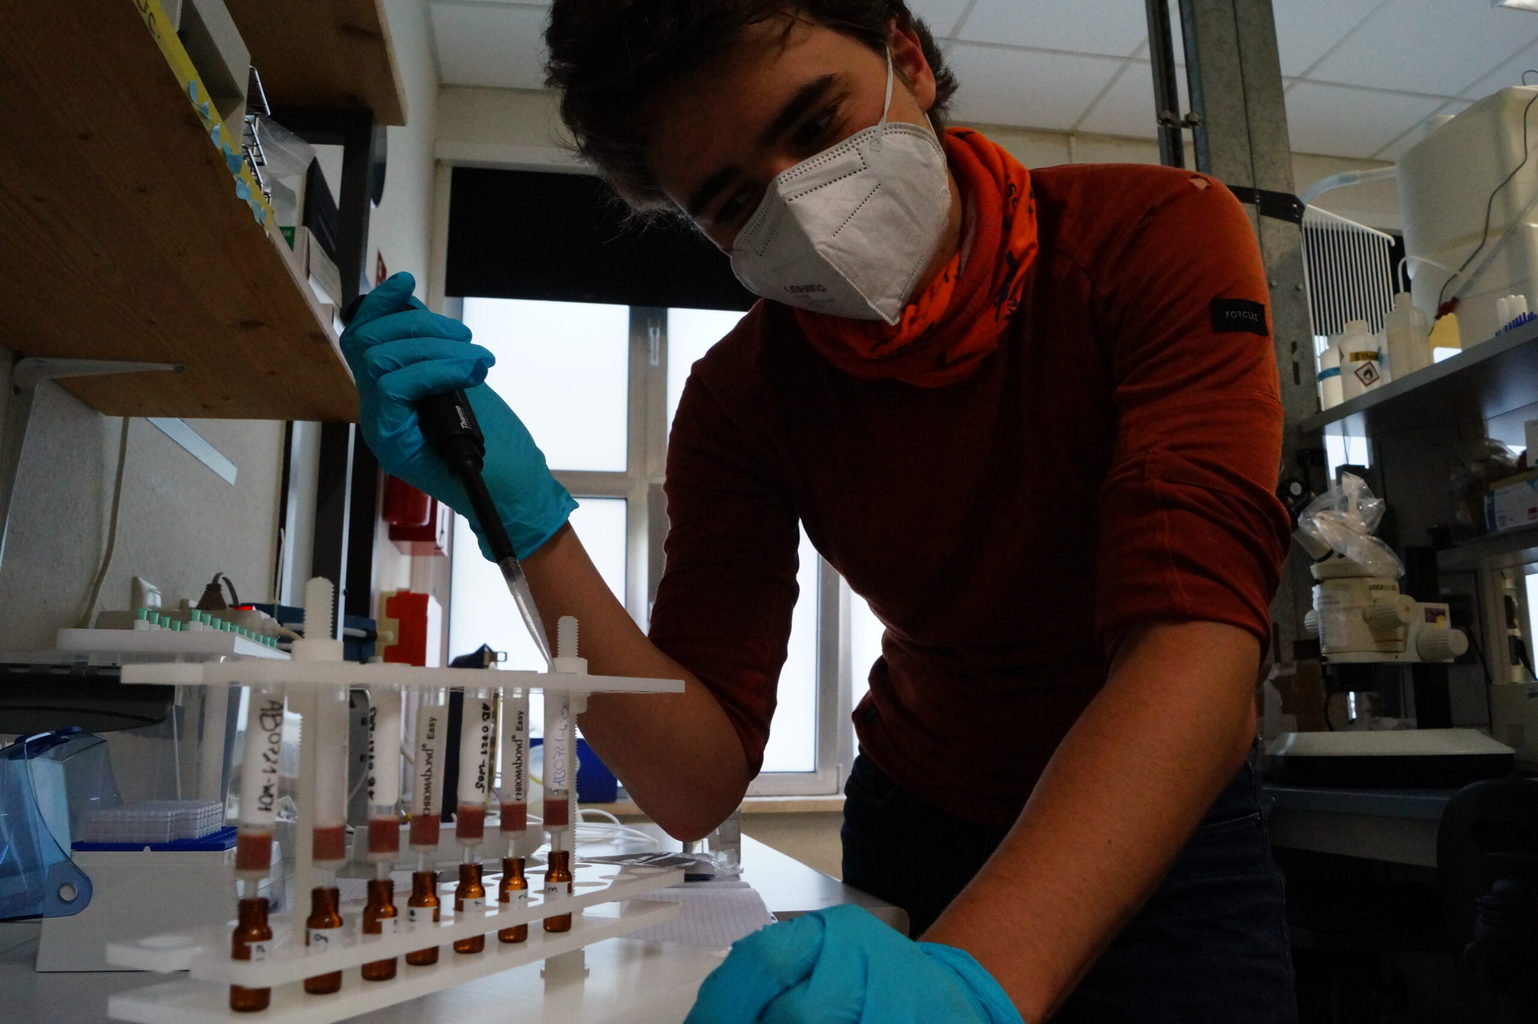
\includegraphics[width=0.8\linewidth]{Bilder/DSC05766-scaled.jpg}
    \caption{Vorbereitung der Wasserproben für den Ionenaustauschchromatographen}
    \label{fig:praep}
\end{figure}